\chapter{运行方式及效果}

\section{客户端运行方式}
\begin{itemize}
    \item 开发环境:macOS Mojave 10.14.5
    \item Android Studio版本:3.4
    \item 项目运行手机版本:小米 MIX 2S
\end{itemize}

\section{服务器运行方式}
\begin{itemize}
    \item 开发环境:macOS Mojave 10.14.5
    \item 运行环境:整个服务器项目在具有v4/v6双栈网络的Centos服务器上编译运行
    \item 运行方式:采用Cmake编译运行方式
\end{itemize}

\newpage
\section{最终项目效果}
连接服务器前后界面如图6.1,6.2所示:
\begin{figure}[!ht]
	\begin{center}
	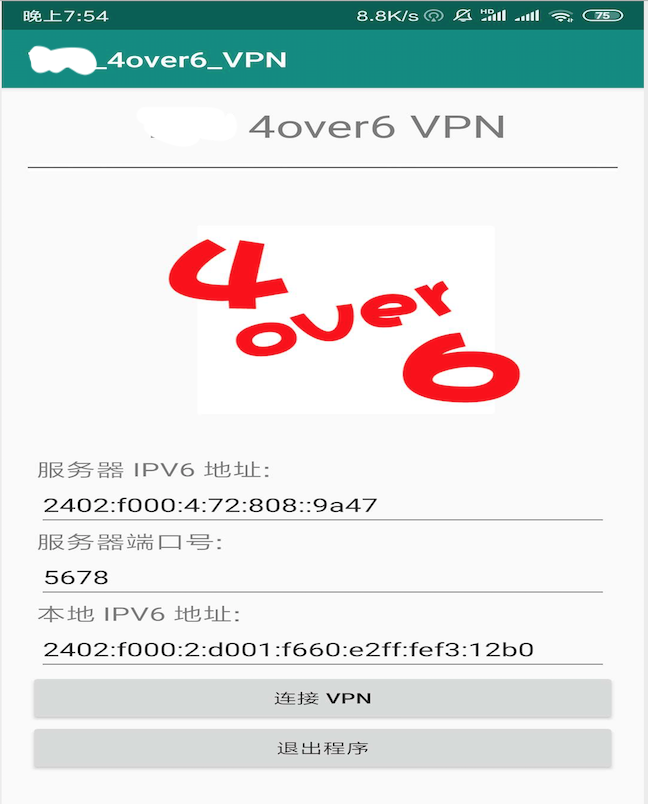
\includegraphics[scale=.58]{connect1.png}
	\end{center}
	\caption{连接服务器前界面}
	\label{figure:连接服务器前界面}
\end{figure}

\begin{figure}[!ht]
	\begin{center}
	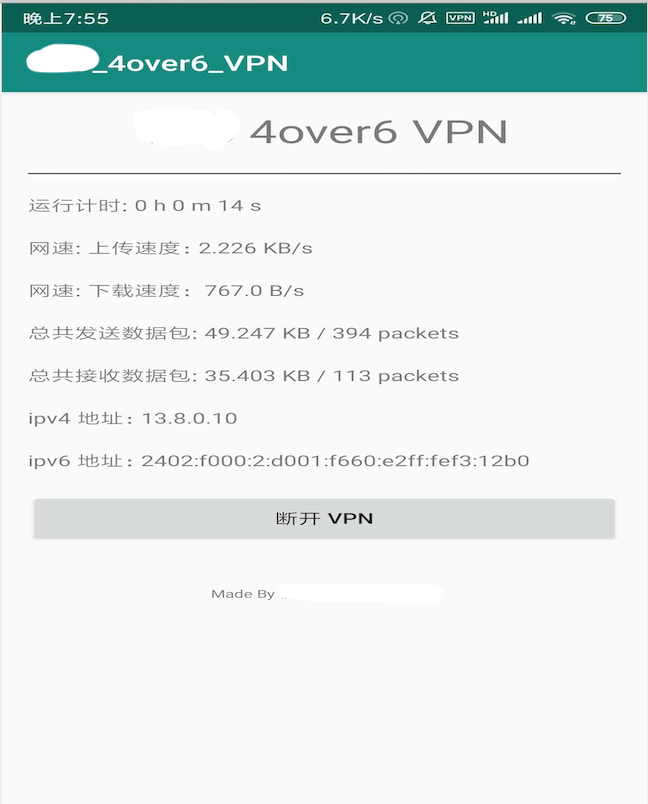
\includegraphics[scale=.58]{connect2.png}
	\end{center}
	\caption{连接服务器后界面}
	\label{figure:连接服务器后界面}
\end{figure}

连接宿舍IPv6网络(未认证账户),使用客户端连接服务器之后访问IPv6网站效果如下:
\begin{figure}[!ht]
	\begin{center}
	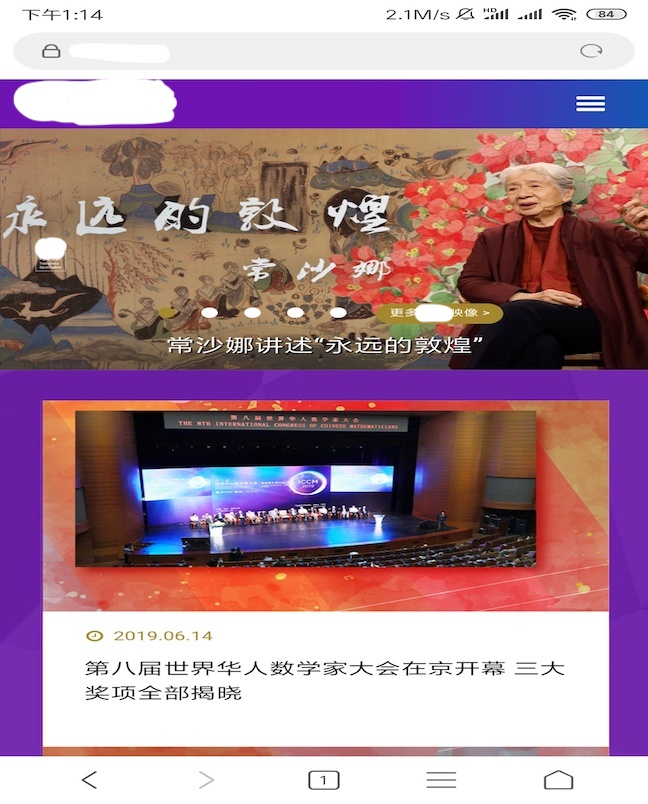
\includegraphics[scale=.58]{tsinghua.jpeg}
	\end{center}
	\caption{访问IPv6网站}
	\label{figure:访问IPv6网站}
\end{figure}

\newpage
连接宿舍IPv6网络(未认证账户),使用客户端连接服务器之后访问IPv4网站效果如下:
\begin{figure}[!ht]
	\begin{center}
	
\includegraphics[scale=.58]{baidu.jpeg}
	\end{center}
	\caption{访问IPv4网站}
	\label{figure:访问IPv4网站}
\end{figure}